%\setcounter{chapter}{9}
\chapter{Communication}

Different communications are detailed in this chapter, such as particle and 
frontier communications.

\section{Particle communication}

When the particles are moved, due to the interaction with the electric field and 
the magnetic field, their position can exceed the boundaries of the chunk where 
they reside. After updating the position of each particle, the ones that exceed 
the chunk must be translated to the correct one. The process of particle 
communication is done in two stages: first the particles are moved in the X 
dimension, then in the Y. Several steps are required in each stage.

\subsection{Exchange in X}
%TODO Place figure to describe the movement
All chunks in the X dimension reside in one MPI process, so the exchange of 
particles can be done by shared memory. Care must be taken to avoid concurrent 
writes in the same chunk by different tasks. The proposed solution avoids the 
problem by using temporal queues in each chunk. The process can be described in 
the following steps:
%
\begin{enumerate}
\item \texttt{collect\_particles\_x}: Out of bound particles in the X direction 
are extracted from the chunk and placed in the correct target chunk queue for 
local exchange.
\item \texttt{exchange\_particles\_x}: Each chunk looks for particles in the 
neighbour chunks target queues and moves them to itself.
\end{enumerate}
%
Usually only two target queues are required for each chunk, as the particles can 
only move one chunk per iteration. However, in the initial iteration after the 
initialization of the particle positions, they can move to any other chunk, and 
the process is subsequently more computationally expensive. We will only focus 
in the general case involving only the two neighbours, as the initialization 
iteration can be disregarded when comparing the time against the whole 
simulation.

% TODO:Should we split this details in another section/chapter involving only
% tasks and TAMPI?
The execution order and mutual exclusion of these two phases should be 
guaranteed by means of a synchronization mechanism. Each step can be implemented 
using OmpSs-2 tasks with dependencies, in order to exploit local parallelism.  
One task collects the particles out of the chunk in the corresponding queues, so 
it needs to access only the current chunk.
%
\begin{lstlisting}
for(i = 0; i < plasma->nchunks; i++)
{
	chunk = &plasma->chunks[i];
	/* Place each particle outside a chunk in the X dimension, in
	 * the lout list */
	#pragma oss task inout(*chunk) label(collect_particles_x)
	for(is = 0; is < sim->nspecies; is++)
	{
		collect_particles_x(sim, chunk, is, global_exchange);
	}
}
\end{lstlisting}
%
The execution of the corresponding exchange particle tasks will start only if 
the collecting step has finished in the neighbour chunks, as otherwise the 
queues are still being written. These dependencies must be placed in all the 
involved chunks.
%
\begin{lstlisting}
for (i = 0; i < plasma->nchunks; i++)
{
	chunk = &plasma->chunks[i];
	...

	#pragma oss task inout(*chunk) \
@          inout(*prev_chunk) inout(*next_chunk) \
@          label(exchange_particles_x)
	{
		/* Only the two neighbours are needed */
		concat_particles(chunk, prev_chunk);
		concat_particles(chunk, next_chunk);
	}
}
\end{lstlisting}
%
Notice that in the first iteration the exchange step must wait for all the 
collecting tasks to finish, as the particles can be moved to any chunk, and thus 
we expect to see a slower iteration than the rest of the simulation. In the 
following steps, only the neighbours at $i-1$, $i$ and $i+1$ are required to 
finish the exchange process.

\begin{figure}[h]
	\centering
	\subfloat[Chain of dependencies observed]{
		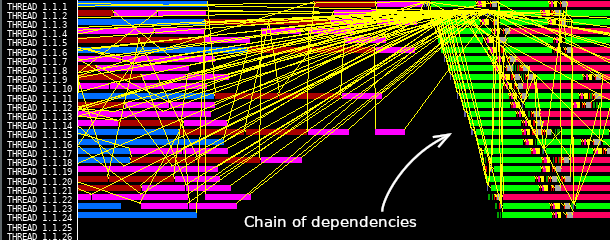
\includegraphics[width=0.7\textwidth]{chain}
		\label{fig:chain}
	}
	\\
	\subfloat[The chain has been corrected]{
		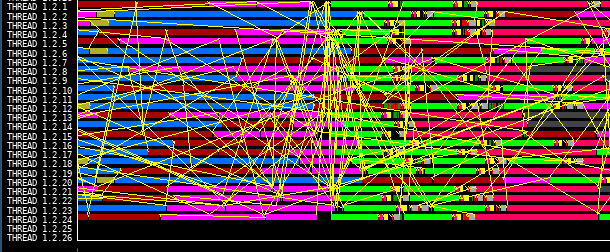
\includegraphics[width=0.7\textwidth]{no-chain}
		\label{fig:no-chain}
	}
	\caption{Comparison of two \texttt{paraver} traces using coloring tasks for 
	communication.}
\end{figure}
%
However, there is a problem with the previous loop: as we create the 
dependencies with the next chunk before the next task is created, we are 
building a chain of dependencies which leads to a sequential execution.  Using 
\texttt{paraver} we can clearly see the chain in the trace graph, shown in the 
figure~\ref{fig:chain}, where no task can run in parallel until the previous one 
finishes.  One solution to alleviate this problem is the use of a coloring 
technique, where each task is assigned a color.  Then all tasks of the same 
color are created first, then the ones with the next color and so on.
%
\begin{figure}[ht]
\centering
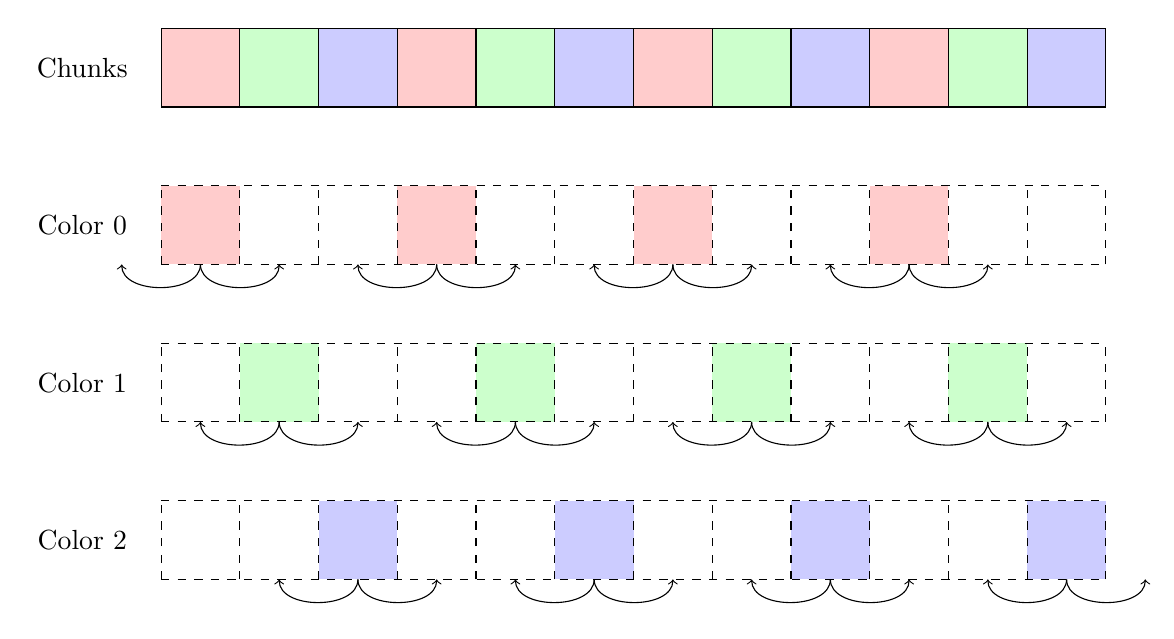
\begin{tikzpicture}
\node at (-1,2.5) {Chunks};
\foreach \x in {0,3,...,9} {
	\fill[red!20](\x,2) rectangle +(1,1);
	\fill[green!20](\x+1,2) rectangle +(1,1);
	\fill[blue!20](\x+2,2) rectangle +(1,1);
}
\draw[step=1] (0,2) grid +(12,1);

\foreach \y\mycol [evaluate=\y as \yy using int(\y/2)]
	in {0/red,2/green,4/blue} {
	\node at (-1,-\y+0.5) {Color \yy};
	\foreach \x in {0,3,...,9} {
		\fill[\mycol!20](\x+\yy,-\y) rectangle +(1,1);
	}
	\foreach \x in {0,3,...,9} {
		\draw[->] (\x,-\y)++(\yy,0)++(.5,0) to[out=-90,in=-90] +(1,0);
		\draw[->] (\x,-\y)++(\yy,0)++(.5,0) to[out=-90,in=-90] +(-1,0);
	}
	\draw[step=1,dashed] (0,-\y) grid +(12,1);
}
%\draw[dashed,step=0.5] (0,0) grid (8,-0.5);
%\draw[thick](0,0) rectangle (8,4);
%
%\fill[white, radius=0.8](4,2) circle;
%\node (center) at (4,2) {\huge $E_y$};
%
%\coordinate (ghost) at (-0.1, -0.25);
%\node (g0r) [left of=ghost, xshift=-0.2cm] {Ghost};
%\draw[->] (g0r) -- (ghost0);
%
%\coordinate (gghost) at (8.1, -0.25);
%\node (ggr) [white,right of=gghost, xshift=0.2cm] {Ghost};
%\draw[white,->] (ggr) -- (gghost);
\end{tikzpicture}
\caption{The coloring technique shown with 12 chunks were the 12 tasks are 
created with 3 colors.}
\label{fig:coloring}
\end{figure}
%
With three colors we ensure that the two tasks of the same color can run in 
parallel without concurrent access to the same chunk, as can be seen in the 
figure~\ref{fig:coloring}.
%
\begin{lstlisting}
max_color = 3;

for(color = 0; color < max_color; color++)
{
	/* Use coloring to prevent a chain of dependencies */
	for(i = color; i < plasma->nchunks; i+=max_color)
	{
		chunk = &plasma->chunks[i];
		...

		#pragma oss task inout(*chunk) \
	@              inout(*prev_chunk) inout(*next_chunk) \
	@              label(collect_local_particles)
		{
			/* Only the two neighbours are needed */
			concat_particles(chunk, prev_chunk);
			concat_particles(chunk, next_chunk);
		}
	}
}
\end{lstlisting}
%
In the figure~\ref{fig:no-chain} it can be observed how the chain has now 
disappeared, and the gaps are now fully covered by tasks running in parallel.

This technique can be expressed without extra work, by using the directive 
\texttt{commutative}, which acts similarly as \texttt{inout} but can be executed 
in any order. Then, once a task begins execution, locking the next chunk, other 
unordered chunk can be executed in any order, if their neighbour chunks are 
unlocked.
%
\begin{lstlisting}
for(i = 0; i < plasma->nchunks; i++)
{
	chunk = &plasma->chunks[i];
	...

	#pragma oss task commutative(*chunk, *prev_chunk, *next_chunk) \
@              label(collect_local_particles)
	{
		/* Only the two neighbours are needed */
		concat_particles(chunk, prev_chunk);
		concat_particles(chunk, next_chunk);
	}
}
\end{lstlisting}
%
Once all exchange tasks are completed, all particles are now placed in the 
correct chunk in the X dimension, and only the Y movement is left.

\subsection{Exchange in Y}
%TODO Place figure to describe the movement
Once the particles are placed in the correct chunk in the X dimension, the 
displacement to the correct chunk in the Y dimension involves sending the 
particles to another MPI process. The steps can be resumed as
%
\begin{enumerate}
\item \texttt{collect\_particles\_y}: Place each particle out of the chunk 
bounds in a queue (one for each target destination).
\item \texttt{pack\_particles\_y}: Pack the particles to be sent to the 
neighbour chunk in a message.
\item \texttt{send\_particles\_y}: Send the packed particles to each neighbour.
\item \texttt{recv\_particles\_y}: Receive the message with the packed 
particles.
\item \texttt{unpack\_particles\_y}: Unpack the particle message and place the 
particles in the chunk.
\end{enumerate}
%
\begin{figure}
\centering
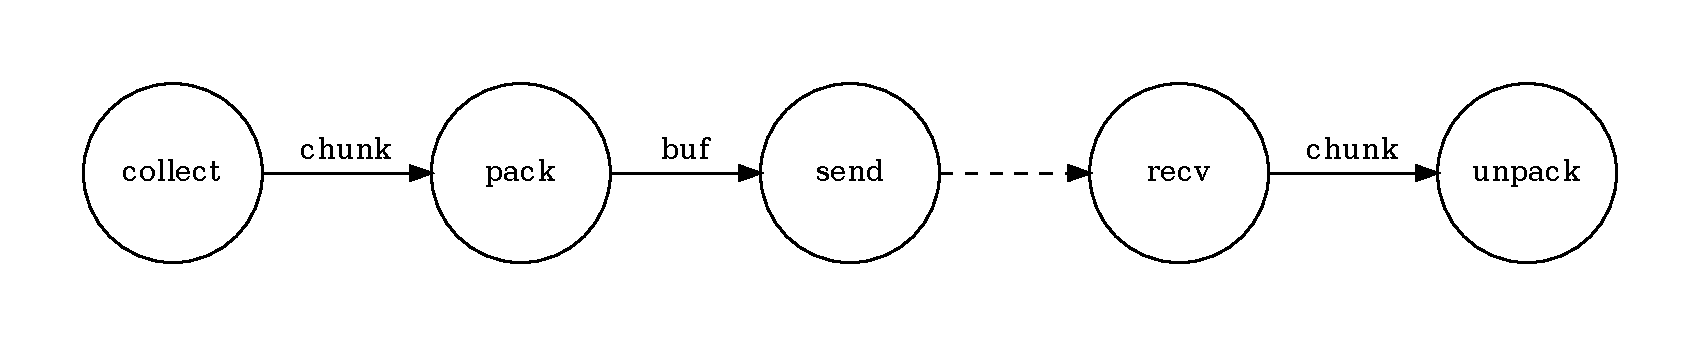
\includegraphics[width=\textwidth]{comm-particles.pdf}
\caption{Graph of task and dependencies of particle communication in Y: Solid 
arrows indicate a data dependency, dashed arrows show a creation dependency 
order.}
\label{fig:comm_y}
\end{figure}
%
Similarly as for the horizontal direction, the particles exceeding the limits of 
each chunk in the Y dimension are placed in a queue.  Once the particles are 
identified within a chunk, they are packed in a message in a contiguous memory 
region. This buffer is then sent using \texttt{MPI\_Send} to the neighbour 
process.

The reception process works in the opposite order: each chunk receives the 
communication of the neighbour chunks in the vertical direction. Once a message 
is received is unpacked and the particles are added to the chunk. In the 
diagram~\ref{fig:comm_y} the dependencies of each step are shown in a graph.

Notice that all the MPI communication is independent of the neighbour chunks in 
the horizontal direction, and can be fully parallelized. Some constraints must 
be added to coordinate the vertical communications to guarantee that no 
simultaneous writes occur in the same chunk.

\begin{lstlisting}
for(i = 0; i < plasma->nchunks; i++)
{
	chunk = &plasma->chunks[i];

	/* Collect particles in a queue that need to change chunk */
	#pragma oss task inout(*chunk) label(collect_particles_y)
	for(is = 0; is < sim->nspecies; is++)
	{
		collect_particles_y(sim, chunk, is, global_exchange);
	}

	/* Prepare the packet to be sent to the neighbour */
	#pragma oss task inout(*chunk) label(pack_particles_y)
	pack_particles_y(sim, chunk, i, global_exchange);

	/* Finally send the packet */
	#pragma oss task in(*chunk) label(send_particles_y)
	send_particles_y(sim, chunk, i, global_exchange);

	/* We cannot create here a task as we don't know the dependencies
	 * when using MPI */
	recv_particles_y(sim, chunk, global_exchange);
}
\end{lstlisting}

\subsection{Mitigation of deadlocks with TAMPI}

Exchanging particles between processes is slightly different when using MPI or 
TAMPI. With the former, the design must be done with special care to avoid 
deadlocks: Assume each chunk tags the message with the chunk index, so the 
receiver can filter messages which are not from the vertical direction. Also, 
consider that we have multiple chunks, more than the number of CPUs available, 
so there are some task that cannot run in parallel and must wait.

It may happen that some task already sent messages and has reached the reception 
stage: it is waiting to continue and subsequently blocking the task until a 
message with the correct tag arrives. But other tasks may be waiting for the CPU 
to begin the communication and didn't send yet any message. When no CPUs are 
left, a deadlock is produced as represented in the 
figure~\ref{fig:comm_deadlock}, where each chunk is represented by a box node 
and the edges show which messages were sent.
%
\begin{figure}
\centering
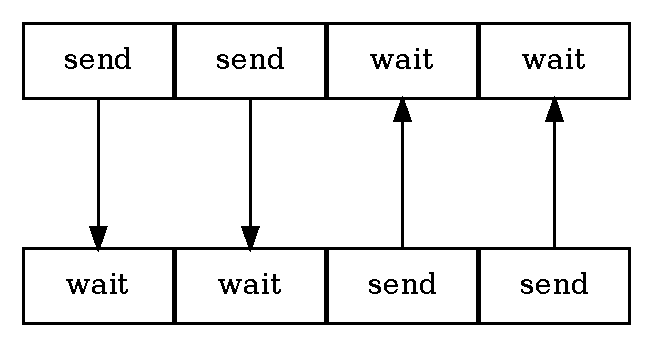
\includegraphics[width=0.4\textwidth]{deadlock-particles.pdf}
\caption{Deadlock at particle exchange in Y, where each message has a different 
tag.}
\label{fig:comm_deadlock}
\end{figure}

In order to palliate the deadlock using only MPI, we can avoid using the tag as 
a filter, so once the sending is complete, the task waits for the reception of 
particles from any other chunk.  With this method, it is guarantee that no 
deadlock can occur, as before a task enters the waiting state, after sending the 
message, another task will be unlocked and can resume the execution:
%
\begin{lstlisting}
#pragma oss task inout(*chunk) weakinout(chunk[0:Nc-1]) \
@    commutative(*sim) label(recv_particle_packet_MPI)
{
	comm_packet_t *pkt;
	...

	MPI_Probe(MPI_ANY_SOURCE, tag, MPI_COMM_WORLD, &status);

	source = status.MPI_SOURCE;
	MPI_Get_count(&status, MPI_BYTE, &size);

	pkt = safe_malloc(size);

	MPI_Recv(pkt, size, MPI_BYTE, source, tag, MPI_COMM_WORLD,
			MPI_STATUS_IGNORE);

	recv_chunk = &sim->plasma.chunks[pkt->dst_chunk[X]];

	#pragma oss task inout(*pkt) inout(*recv_chunk) label(unpack_comm_packet)
	{
		unpack_comm_packet(sim, recv_chunk, pkt);
		free(pkt);
	}
}
\end{lstlisting}
%
It must be enforced that the calls to \texttt{MPI\_Recv} and \texttt{MPI\_Probe} 
are done in mutual exclusion, as otherwise another task could receive the 
message between the tho calls. The dependency with the sentinel \texttt{*sim} 
avoids the problem, which is released as soon as the packet is received. Notice 
that, in order to create a nested task to process the chunk stated in the 
packet, we must indicate in the \texttt{weakinout} directive all posible chunks 
that may be selected. Then, only one will be used by the child task to unpack 
the particles.

The downside of the described mechanism is the implicit complexity and the 
amount of extra work needed to ensure a deadlock free execution, which can be 
avoided with TAMPI. The deadlock is mitigated not by removing the tag, which 
filters the chunk, but by setting the task to sleep once it enters in the 
waiting state, so other tasks can begin the execution. The TAMPI library 
intercepts the calls to MPI and informs the OmpSs-2 scheduler that the task can 
be put to sleep.

Using TAMPI only requires a minor modifications with respect to the original 
implementation: the message size must be known at the receiver. The current 
version of TAMPI doesn't include \texttt{MPI\_Probe} in the family of 
intercepted functions. The MPI version first probes for the message to get the 
length and then allocates a buffer to hold the entire message. A buffer of known 
size may be used to hold the parts of the message while is being send. The 
message includes the complete size of the message in the header, so after the 
reception of the first message, the whole buffer can be allocated.

\begin{lstlisting}
#pragma oss task out(*pkt) inout(*chunk) label(recv_particle_packet_TAMPI)
{
	...

	size = BUFSIZE;
	pkt = safe_malloc(size);
	MPI_Recv(pkt, size, MPI_BYTE, proc, tag, MPI_COMM_WORLD,
			MPI_STATUS_IGNORE);

	/* If more data is comming, realloc and receive it */
	if(pkt->size > size)
	{
		done = size;
		size = pkt->size;
		parts_left = (size - done + (BUFSIZE - 1)) / BUFSIZE;

		/* If the packet is only a fragment, continue until we
		 * fill the whole buffer */
		pkt = realloc(pkt, size);
		if(!pkt) abort();

		requests = safe_malloc(parts_left * sizeof(MPI_Request));

		/* Recv by chunks */
		for(j=0,ptr=pkt,i=BUFSIZE; i<size; j++, i+=BUFSIZE)
		{
			left = size - i;
			if(left > BUFSIZE)
				left = size;

			MPI_Irecv(ptr+i, left, MPI_BYTE, proc, tag,
					MPI_COMM_WORLD, &requests[j]);
		}

		MPI_Waitall(parts_left, requests, MPI_STATUSES_IGNORE);
		free(requests);
	}
	unpack_comm_packet(sim, chunk, pkt);
	free(pkt);
}
\end{lstlisting}

Note that all communications are done with \texttt{MPI\_BYTE}, sending the 
packed structures as an array of bytes. This methods of transmission sends the 
data ``as-is''---MPI doesn't perform any endianness adjustment. We assume the 
simulation will run within nodes with the same endianness, otherwise MPI will 
need information of each field or a manual process must be added before the 
message is unpacked. Additionally, the structures sent over MPI are packed to 
avoid any holes in the buffer sent.

\section{Field communication}

Each MPI process holds a block with the different fields of the assigned region 
of space. Due to the interpolation process some elements of the neighbour fields 
are needed to complete the interpolation, which implies that additional 
communication is needed.

\subsection{Charge density $\rho$}

Following the order of the simulation, first the $\rho$ field is updated, where 
all particles deposit the charge. Given a $\rho$ field of size $(n_x, n_y)$ an 
extra row $\rho_{n_y}$ is added to hold the first row of $\rho$ of the next 
block $\rho_0$, as shown in the figure~\ref{fig:field_rho}. Notice that an extra 
padding is required by the FFTW library, to accommodate intermediate results, 
and must be taken into account when designing the communications.
%
\begin{figure}[ht]
\centering
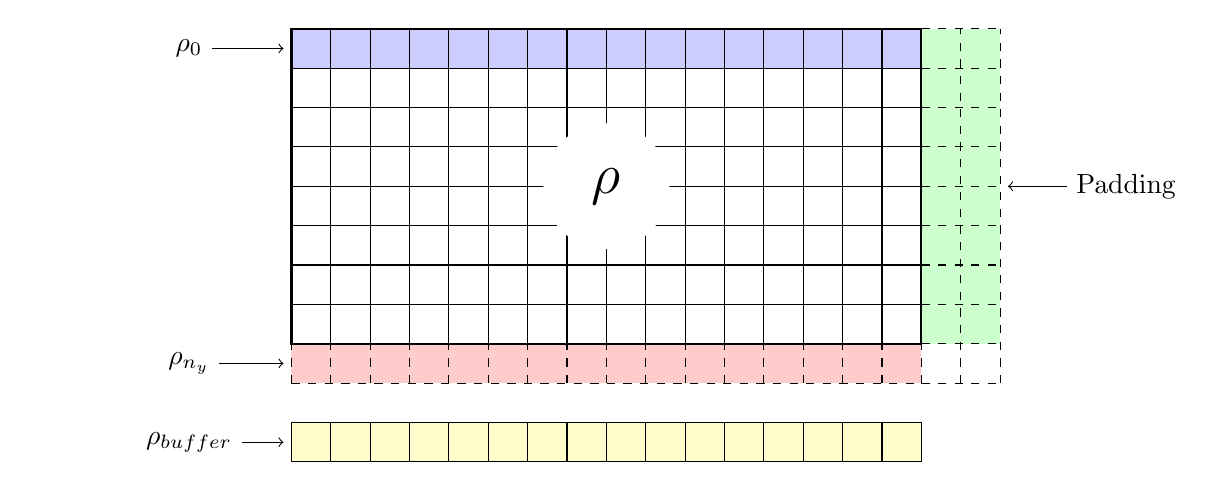
\begin{tikzpicture}
\fill[blue!20](0,3.5) rectangle (8,4);
\draw[step=0.5] (0,0) grid (8,4);
\fill[red!20](0,0) rectangle (8,-0.5);
\draw[dashed,step=0.5] (0,0) grid (8,-0.5);
\fill[green!20](8,0) rectangle (9,4);
\draw[dashed,step=0.5] (8,-0.5) grid (9,4);
\draw[thick](0,0) rectangle (8,4);

\coordinate (first) at (-0.1, 3.75);
\fill[white, radius=0.8](4,2) circle;
\node (center) at (4,2) {\huge $\rho$};
\node (fr) [left of=first, xshift=-0.2cm] {$\rho_0$};
\draw[->] (fr) -- (first);

\coordinate (ghost) at (-0.1, -0.25);
\node (gr) [left of=ghost, xshift=-0.2cm] {$\rho_{n_y}$};
\draw[->] (gr) -- (ghost);

\coordinate (fft) at (9.1, 2);
\node (fft-label) [right of=fft, xshift=0.5cm] {Padding};
\draw[->] (fft-label) -- (fft);

\coordinate (gfft) at (-1.1, 2);
\node (gfft-label) [white,left of=gfft, xshift=-0.5cm] {Padding};
\draw[white,->] (gfft-label) -- (gfft);

\fill[yellow!20](0,-1) rectangle (8,-1.5);
\draw[step=0.5] (0,-1) grid (8,-1.5);
\coordinate (buf) at (-0.1, -1.25);
\node (br) [left of=buf, xshift=-0.2cm] {$\rho_\text{buffer}$};
\draw[->] (br) -- (buf);
\end{tikzpicture}
\caption{The field $\rho$ with the padding}
\label{fig:field_rho}
\end{figure}

Each process sends $\rho_{n_y}$ to the next process, and receives $\rho_0$ from 
the previous one. The size of the message is constant and known beforehand, so 
it can the be stored in the same buffer $\rho_\text{buffer}$ in each iteration, 
which is added to $\rho_0$ to finally complete $\rho$ where the ghost is no 
longer needed.

If the ghost is sent before we begin the reception process, we can reuse 
$\rho_{n_y}$ to hold also $\rho_\text{buffer}$. But the communications use 
non-blocking communications, which may not finish when the process reaches the 
reception step, so an additional buffer is used instead---a technique known as 
double buffering.  Before each send the status of the previous request is 
tested, and in case is not yet finished, we wait before continue. The two main 
functions \texttt{comm\_mat\_send} and \texttt{comm\_mat\_recv} are used to 
transfer a buffer of floating point numbers.

\begin{lstlisting}
int comm_mat_send(sim_t *sim, double *data, int size, int dst,
	int op, int dir, MPI_Request *req)
{
	int tag = compute_tag(op, sim->iter, dir, COMM_TAG_DIR_SIZE);

	if(*req)
		MPI_Wait(req, MPI_STATUS_IGNORE);

	return MPI_Isend(data, size, MPI_DOUBLE, dst, tag,
		MPI_COMM_WORLD, req);
}

int comm_mat_recv(sim_t *sim, double *data, int size, int dst,
	int op, int dir)
{
	int tag = compute_tag(op, sim->iter, dir, COMM_TAG_DIR_SIZE);

	return MPI_Recv(data, size, MPI_DOUBLE, dst, tag,
		MPI_COMM_WORLD, MPI_STATUS_IGNORE);
}
\end{lstlisting}

\subsection{Electric potential $\phi$}

After the solver, the result is stored in a similar way as $\rho$, with padding 
at the right. However, now we have more ghosts at the top and at the bottom of 
$\phi$, as they will be needed to compute the electric field $\E$. In the 
figure~\ref{fig:field_phi} the different regions can be seen: In blue the ones 
which will be send, $\phi_{0}$ and $\phi_{1}$ to the previous process to fill 
$\varphi_{n_y}$ and $\varphi_{n_y + 1}$, and $\phi_{n_y - 1}$ to be sent to the 
next process, to fill $\varphi_{-1}$.
%
\begin{figure}[ht]
\centering
\begin{tikzpicture}
\fill[red!20](0,4) rectangle (8,4.5);
\draw[dashed,step=0.5] (0,4) grid (8,4.5);
\fill[blue!20](0,3) rectangle (8,4);
\fill[blue!20](0,0) rectangle (8,0.5);
\draw[step=0.5] (0,0) grid (8,4);
\fill[red!20](0,0) rectangle (8,-1);
\draw[dashed,step=0.5] (0,0) grid (8,-1);
\fill[green!20](8,0) rectangle (9,4);
\draw[dashed,step=0.5] (8,-1) grid (9,4.5);
\draw[thick](0,0) rectangle (8,4);

\fill[white, radius=0.8](4,2) circle;
\node (center) at (4,2) {\huge $\phi$};

\coordinate (first) at (-0.1, 3.75);
\node (fr) [left of=first, xshift=-0.2cm] {$\phi_0$};
\draw[->] (fr) -- (first);

\coordinate (second) at (-0.1, 3.25);
\node (sr) [left of=second, xshift=-0.2cm] {$\phi_1$};
\draw[->] (sr) -- (second);

\coordinate (last) at (-0.1, 0.25);
\node (sr) [left of=last, xshift=-0.2cm] {$\phi_{n_y - 1}$};
\draw[->] (sr) -- (last);

\coordinate (ghost-1) at (-0.1, 4.25);
\node (g-1r) [left of=ghost-1, xshift=-0.2cm] {$\varphi_{-1}$};
\draw[->] (g-1r) -- (ghost-1);
\coordinate (ghost0) at (-0.1, -0.25);
\node (g0r) [left of=ghost, xshift=-0.2cm] {$\varphi_{n_y}$};
\draw[->] (g0r) -- (ghost0);
\coordinate (ghost1) at (-0.1, -0.75);
\node (g1r) [left of=ghost1, xshift=-0.2cm] {$\varphi_{n_y + 1}$};
\draw[->] (g1r) -- (ghost1);

\coordinate (fft) at (9.1, 2);
\node (fft-label) [right of=fft, xshift=0.5cm] {Padding};
\draw[->] (fft-label) -- (fft);

\coordinate (gfft) at (-1.1, 2);
\node (gfft-label) [white,left of=gfft, xshift=-0.5cm] {Padding};
\draw[white,->] (gfft-label) -- (gfft);

\end{tikzpicture}
\caption{The electric potential $\phi$ with the ghost rows (red) and padding 
(green)}
\label{fig:field_phi}
\end{figure}
%
Notice the use of the notation $\varphi$ to denote the ghosts and $\phi$ the 
rows of the actual field.

It can be observed that the first two rows $\phi_0$ and $\phi_1$ are not 
consecutive in memory, as they have the padding at the right. To avoid two 
messages or additional copies, the two rows are sent with the padding included, 
which will be placed ``as-is'' in the receiving process at $\varphi_{n_y}$ and 
$\varphi_{n_y + 1}$, as the padding region is ignored.

\subsection{Electric field $\boldsymbol{E}$}

The electric field $\E$ can be computed from the ghosts of the electric 
potential $\phi$ without the need of extra communications. The electric field 
$E_x$ with a periodic boundary is obtained from $\phi$, as the whole space 
domain is available in the block in the $X$ dimension.
%
\begin{figure}[ht]
\centering
\begin{tikzpicture}
\draw[step=0.5] (0,0) grid (8,4);
\fill[red!20](0,0) rectangle (8,-0.5);
\draw[dashed,step=0.5] (0,0) grid (8,-0.5);

\fill[white, radius=0.8](4,2) circle;
\node (center) at (4,2) {\huge $E_y$};

\coordinate (ghost) at (-0.1, -0.25);
\node (g0r) [left of=ghost, xshift=-0.2cm] {$\mathcal{E}_y(n_y)$};
\draw[->] (g0r) -- (ghost0);

\coordinate (gghost) at (8.1, -0.25);
\node (ggr) [white,right of=gghost, xshift=0.2cm] {Ghost};
\draw[white,->] (ggr) -- (gghost);
\draw[thick](0,0) rectangle (8,4);

\end{tikzpicture}
\caption{The electric field $E_y$ with the ghost row at $n_y$ (red)}
\label{fig:field_Ey}
\end{figure}
%
In the case of $E_y$ we will need the ghost row at $n_y$, which is marked in red 
in the figure~\ref{fig:field_Ey}, in order to interpolate the electric field in 
the particles of the block. But the computation of the whole field can be 
produced from the extra ghost rows stored in $\phi$, which were precisely placed 
to avoid another communication step.
